\documentclass[11pt,letterpaper]{article}
\usepackage[lmargin=1in,rmargin=1in,tmargin=1in,bmargin=1in]{geometry}
\usepackage{../style/homework}
\usepackage{../style/commands}
\setbool{quotetype}{false} % True: Side; False: Under
\setbool{hideans}{false} % Student: True; Instructor: False

\newcommand{\xor}{\,\underline{\vee}\,}

% Logical Circuits
\usepackage{circuitikz}
\usetikzlibrary{shapes.gates.logic.US,shapes.gates.logic.IEC}

% -------------------
% Content
% -------------------
\begin{document}

\homework{2: Due 09/12}{I am very seldom interested in applications. I am more interested in the elegance of a problem. Is it a good problem, an interesting problem?}{Claude Shannon}

% Problem 1
\problem{10} Often, one encounters expressions along the lines, ``This happens, unless this.'' In symbolic form, we could write this as, ``$P$ happens, unless $Q$.'' Most often, what is meant by this is, ``if $\neg Q$, then $P$.'' That is, ``$P$ unless $Q$'' means $\neg Q \to P$. 
	\begin{enumerate}[(a)]
	\item Consider the statement, ``Payment is due on fifth of the month, unless it is a weekend.'' Rewrite this statement in ``if\dots then'' form.  
	\item Write the negation of ``Payment is due on fifth of the month, unless it is a weekend'' as a complete English sentence. 
	\item Is payment not being due a sufficient condition for the fifth being the weekend? Explain. 
	\item Is the fifth of the month being a weekend sufficient for payment not being due? Explain. 
	\end{enumerate} 

\sol 
\begin{enumerate}[(a)]
\item 
%\item From the problem statement (and from thinking about how we use language), we can see that the statement, ``Payment is due on fifth of the month, unless it is a weekend,'' is equivalent to the sentence, ``If the fifth is not a weekend, then payment is due on the fifth.'' Alternatively, choose $P$ to be the proposition, ``Payment is due on the fifth of the month,'' and $Q$ to be the proposition, ``The fifth is a weekend.'' Then the given statement is $P$ unless $Q$. But from the problem statement, we know this is $\neg Q \to P$. As a sentence, this is the statement, ``If the fifth is not a weekend, then payment is due on the fifth.'' 
%
%\item From (a), we know that the statement of the problem is equivalent to $\neg Q \to P$, where $P, Q$ are chosen as in (a). The negation of this is $\neg (\neg Q \to P) \equiv \neg Q \wedge \neg P$. This is the statement, ``The fifth is not a weekend and payment is not due on the fifth of the month.'' 
%
%\item From (a), we know that the statement of the problem is equivalent to $\neg Q \to P$, where $P, Q$ are chosen as in (a). So we know that $\neg Q$ is a necessary condition for $P$, and that $P$ is a sufficient condition for $\neg Q$; that is, the fifth not being a weekend is a necessary condition for payment to be due on the fifth, and payment being due on the fifth is a sufficient condition for the fifth not being a weekend. If payment not being due, i.e. $\neg P$, is a sufficient condition for the fifth being the weekend, i.e. $Q$, then $\neg P \to Q$. Observe that this is the contrapositive of $\neg Q \to P$, which has contrapositive $\neg P \to \neg (\neg Q) \equiv \neg P \to Q$. Therefore, $\neg P \to Q$ and $\neg Q \to P$ have the same truth value. This shows that payment not being due is a sufficient condition for the fifth being a weekend. This should make sense because payment will be due on the fifth, unless it was a weekend. So it is sufficient for payment not being due for the fifth to be the weekend---though it may not be necessary. 
%
%\item From (a), we know that the statement of the problem is equivalent to $\neg Q \to P$, where $P, Q$ are chosen as in (a). So we know that $\neg Q$ is a necessary condition for $P$, and that $P$ is a sufficient condition for $\neg Q$; that is, the fifth not being a weekend is a necessary condition for payment to be due on the fifth, and payment being due on the fifth is a sufficient condition for the fifth not being a weekend. If the fifth of the month being a weekend, i.e. $Q$, is a sufficient condition for payment not to be due on the fifth, i.e. $\neg P$, then $Q \to \neg P$. Observe that $Q \to \neg P \not\equiv$
\end{enumerate}



\newpage



% Problem 2
\problem{10} In everyday speech, ``this or that'' could mean, ``this, that, or both'' or it could mean, ``this, that, but not both.'' Both interpretations are common. ``Mathematical OR'' \textit{always} allows the possibility for both, i.e. $P \vee Q$ is true if $P$ is true, $Q$ is true, or both $P$ and $Q$ are true. It would be advantageous to have an ``exclusive or'' for logical expressions. Define ``mathematical exclusive or'' to be $P \xor Q$; that is, $P \xor Q$ is true when exactly one of $P$, $Q$ is true. 
	\begin{enumerate}[(a)]
	\item Give the logic table for $P \xor Q$
	\item Using a logic table, show that $P \xor Q \equiv (P \wedge \neg Q) \vee (\neg P \wedge Q)$.
	\item Without computing $P \xor Q \iff (P \wedge \neg Q) \vee (\neg P \wedge Q)$, determine whether this proposition is a tautology. Explain. 
	\item Use (b) to find a logical expression for $\neg (P \xor Q)$ in terms of $P$'s, $Q$'s, $\neg$'s, $\wedge$'s, and $\vee$'s; that is, find a `rule' for determining how to negate $P \xor Q$. `Simplify' your expression as much as possible. 	
	\end{enumerate} \pspace

\sol 
\begin{enumerate}[(a)]
\item We know that $P \xor Q$ is true only when exactly one of $P, Q$ is true, i.e. $P \xor Q$ is false if $P$ and $Q$ are both true or when $P$ and $Q$ are both false. This gives us the following truth table: \par
	\begin{table}[h]
	\centering
	\begin{tabular}{ccc}
	$P$ & $Q$ & $P \xor Q$ \\ \hline
	$T$ & $T$ & $F$ \\
	$T$ & $F$ & $T$ \\
	$F$ & $T$ & $T$ \\
	$F$ & $F$ & $F$ 
	\end{tabular}
	\end{table} \pspace

\item We need only show that each output for $P \xor Q$ and $(P \wedge \neg Q) \vee (\neg P \wedge Q)$, no matter the input for $P, Q$. Now we have\dots \par
	\begin{table}[h]
	\centering
	\begin{tabular}{ccccccc}
	$P$ & $Q$ & $\neg P$ & $\neg Q$ & $P \wedge \neg Q$ & $\neg P \wedge Q$ & $(P \wedge \neg Q) \vee (\neg P \wedge Q)$ \\ \hline
	$T$ & $T$ & $F$ & $F$ & $F$ & $F$ & $F$ \\
	$T$ & $F$ & $F$ & $T$ & $T$ & $F$ & $T$ \\
	$F$ & $T$ & $T$ & $F$ & $F$ & $T$ & $T$ \\
	$F$ & $F$ & $T$ & $T$ & $F$ & $F$ & $F$
	\end{tabular}
	\end{table}
Because the output column here, i.e. $(P \wedge \neg Q) \vee (\neg P \wedge Q)$, matches the output column from (a), i.e. $P \xor Q$, we know that $P \xor Q \equiv (P \wedge \neg Q) \vee (\neg P \wedge Q)$. Alternatively, we know that $P \xor Q \equiv (P \wedge \neg Q) \vee (\neg P \wedge Q)$ if both logical expressions are true simultaneously. We know $P \xor Q$ is true only when $P$ is true and $Q$ is false, i.e. $P \wedge \neg Q$, or when $P$ is false and $Q$ is true, i.e. $\neg P \wedge Q$. But this is precisely the right-hand side of the equivalence. \pspace

\item We know that $R \iff S$ is a tautology if and only if $R \equiv S$. From (b), we know that $P \xor Q \equiv (P \wedge \neg Q) \vee (\neg P \wedge Q)$. Therefore, it must be that $P \xor Q \iff (P \wedge \neg Q) \vee (\neg P \wedge Q)$ is a tautology, which is easily verified via a logic table. \pspace

\item We have\dots
	\[
	\begin{gathered}
	\neg (P \xor Q) \\[0.3cm]
	\neg \big( (P \wedge \neg Q) \vee (\neg P \wedge Q) \big) \\[0.3cm]
	\neg (P \wedge \neg Q) \wedge \neg (\neg P \wedge Q) \\[0.3cm]
	\big( \neg P \vee \neg (\neg Q) \big) \wedge \big( \neg (\neg P) \vee \neg Q \big) \\[0.3cm]
	(\neg P \vee Q) \wedge (P \vee \neg Q) \\[0.3cm]
	\big( \neg P \wedge (P \vee \neg Q) \big) \vee \big(Q \wedge (P \vee \neg Q) \big) \\[0.3cm]
	\left( (\neg P \wedge P) \vee (\neg P \wedge \neg Q) \right) \vee \left( (Q \wedge P) \vee (Q \wedge \neg Q) \right) \\[0.3cm]
	\big( F_0 \vee (\neg P \wedge \neg Q) \big) \vee \big( (P \wedge Q) \vee F_0 \big) \\[0.3cm]
	(\neg P \wedge \neg Q) \vee (P \wedge Q) 
	\end{gathered}
	\] \pspace
But then we have `rule' $\neg (P \xor Q) \equiv (\neg P \wedge \neg Q) \vee (P \wedge Q)$. This makes sense as if $P \xor Q$ is true, then exactly one of $P, Q$ is true. But then $\neg (P \xor Q)$ is false. We know $P \xor Q$ is false if $P$ and $Q$ are both false, i.e. $\neg P \wedge \neg Q$, or if $P$ and $Q$ are both true, i.e. $P \wedge Q$, but this is precisely the equivalence we have derived. 
\end{enumerate}



\newpage



% Problem 3
\problem{10} We can use Boolean representations of circuits to simplify circuits and reduce the amount of wire, chips, etc. required. Consider the circuit below:
	\[
	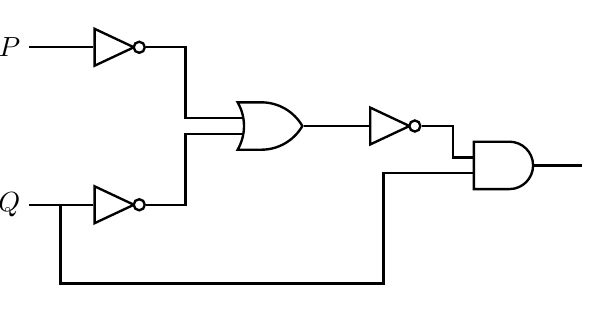
\begin{tikzpicture}
	\node (p) at (0,2) {\hspace{-0.5cm}$P$};
	\node (q) at (0,0) {\hspace{-0.5cm}$Q$};
	
	\node[not gate US, draw, line width= 0.03cm] at (1,2) (not1) {};
	\node[not gate US, draw, line width= 0.03cm] at (1,0) (not2) {};
	\node[not gate US, draw, line width= 0.03cm] at (4.5,1) (not3) {};
	\node[or gate US, draw, line width= 0.03cm] at (3,1) (or1) {};
	\node[and gate US, draw, line width= 0.03cm] at (6,0.5) (and1) {};
	
	\draw[line width= 0.03cm] (p) |- (not1.input);
	\draw[line width= 0.03cm] (q) |- (not2.input);
	
	\draw[line width= 0.03cm] (not1.output) -- ([xshift=0.5cm]not1.output) |- (or1.input 1);
	\draw[line width= 0.03cm] (not2.output) -- ([xshift=0.5cm]not2.output) |- (or1.input 2);
	
	\draw[line width= 0.03cm] (or1.output) |- (not3.input);
	\draw[line width= 0.03cm] (not3.output) -- ([xshift=0.4cm]not3.output) |- (and1.input 1);
	\draw[line width= 0.03cm] (q) |- (0.4,0) |- (0.4,-1) |- (4.5,-1) |- (and1.input 2);
	
	\draw[line width= 0.03cm] (and1.output) |- ([xshift=0.6cm]and1.output);
	\end{tikzpicture}
	\]

\begin{enumerate}[(a)]
\item Find the logical expression corresponding to the given circuit.
\item `Simplify' the logical expression from (a).
\item Sketch the circuit from (b).
\end{enumerate} 

\sol 
\begin{enumerate}[(a)]
\item We can slowly `move through' the circuit, carefully labeling along the way.
	\[
	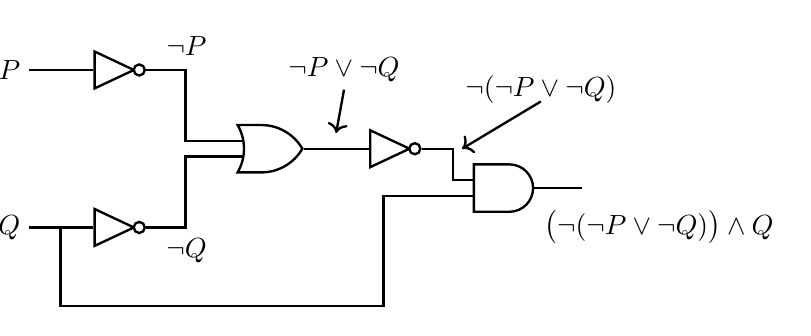
\begin{tikzpicture}
	\node (p) at (0,2) {\hspace{-0.5cm}$P$};
	\node (q) at (0,0) {\hspace{-0.5cm}$Q$};
	
	\node[not gate US, draw, line width= 0.03cm] at (1,2) (not1) {};
	\node[not gate US, draw, line width= 0.03cm] at (1,0) (not2) {};
	\node[not gate US, draw, line width= 0.03cm] at (4.5,1) (not3) {};
	\node[or gate US, draw, line width= 0.03cm] at (3,1) (or1) {};
	\node[and gate US, draw, line width= 0.03cm] at (6,0.5) (and1) {};
	
	\draw[line width= 0.03cm] (p) |- (not1.input);
	\draw[line width= 0.03cm] (q) |- (not2.input);
	
	\draw[line width= 0.03cm] (not1.output) -- ([xshift=0.5cm]not1.output) |- (or1.input 1);
	\draw[line width= 0.03cm] (not2.output) -- ([xshift=0.5cm]not2.output) |- (or1.input 2);
	
	\draw[line width= 0.03cm] (or1.output) |- (not3.input);
	\draw[line width= 0.03cm] (not3.output) -- ([xshift=0.4cm]not3.output) |- (and1.input 1);
	\draw[line width= 0.03cm] (q) |- (0.4,0) |- (0.4,-1) |- (4.5,-1) |- (and1.input 2);
	
	\draw[line width= 0.03cm] (and1.output) |- ([xshift=0.6cm]and1.output);
	
	\node at (2,2.3) {$\neg P$};
	\node at (2,-0.3) {$\neg Q$};
	\node at (4,2) {$\neg P \vee \neg Q$};
	\draw[line width=0.03cm,->] (4,1.75) -- (3.9,1.2);
	\node at (6.5,1.75) {$\neg (\neg P \vee \neg Q)$};
	\draw[line width=0.03cm,->] (6.5,1.6) -- (5.5,1);
	\node at (8,0) {$\big( \neg (\neg P \vee \neg Q) \big) \wedge Q$};
	\end{tikzpicture}
	\]
From the diagram above, we can see that the logical/Boolean expression equivalent to the circuit above is $\big( \neg (\neg P \vee \neg Q) \big) \wedge Q$. \pspace

\item Simplifying the logical expression from (a), we have\dots
	\[
	\begin{gathered}
	\big( \neg (\neg P \vee \neg Q) \big) \wedge Q \\[0.3cm]
	\big( \neg (\neg P) \wedge \neg (\neg Q) \big) \wedge Q \\[0.3cm]
	(P \wedge Q) \wedge Q \\[0.3cm]
	P \wedge (Q \wedge Q) \\[0.3cm]
	P \wedge Q
	\end{gathered}
	\]

\item Building the circuit from the simplified expression in (b), we have\dots
	\[
	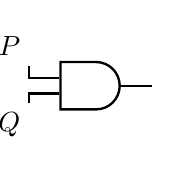
\begin{tikzpicture}
	\node (p) at (0,1) {\hspace{-0.5cm}$P$};
	\node (q) at (0,0) {\hspace{-0.5cm}$Q$};

	\node[and gate US, draw, line width= 0.03cm] at (0.75,0.5) (and1) {};
	
	\draw[line width= 0.03cm] (p) |- (and1.input 1);
	\draw[line width= 0.03cm] (q) |- (and1.input 2);

	\draw[line width= 0.03cm] (and1.output) -- ([xshift=0.4cm]and1.output);
	\end{tikzpicture}
	\]
From the work in (a) and (b), we know that the circuit above has the exact same `behavior', i.e. input-output table, as the circuit in (a)---but with a substantial savings on gates and wiring. 
\end{enumerate}



\newpage



% Problem 4
\problem{10} Draw a circuit diagram corresponding to the logical expression below and construct its input/output table.
	\[
	\neg (P \vee \neg Q) \wedge (P \vee Q)
	\] \pspace

\sol Following `order of operations,' we see that we need to feed $Q$ into a NOT gate. This result must be fed into an OR gate with $P$. This result must then be put into an inverter, which is then fed into an AND gate. We need to construct the other input to the AND gate. For that, we need to feed $P, Q$ into an OR gate. This result is the other input to the final AND gate. This gives us the circuit below. 
	\[
	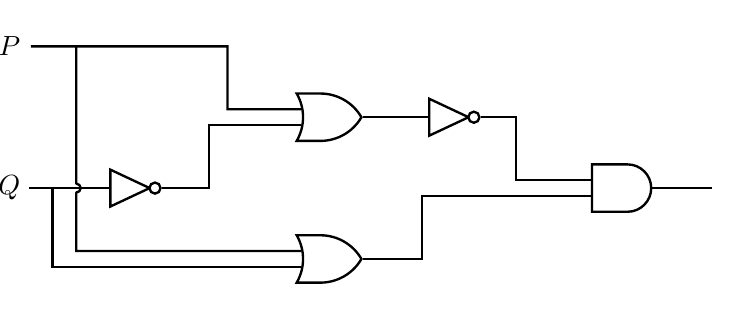
\begin{tikzpicture}[scale=1.5]
	\node (p) at (0,1.2) {\hspace{-0.5cm}$P$};
	\node (q) at (0,0) {\hspace{-0.5cm}$Q$};
	
	\node[not gate US, draw, line width= 0.03cm] at (0.8,0) (not1) {};
	\node[or gate US, draw, line width= 0.03cm] at (2.5,0.6) (or1) {};
	\node[not gate US, draw, line width= 0.03cm] at (3.5,0.6) (not2) {};
	\node[or gate US, draw, line width= 0.03cm] at (2.5,-0.6) (or2) {};
	\node[and gate US, draw, line width= 0.03cm] at (5,0) (and1) {};
	
	\draw[line width= 0.03cm] (p) -- (1.68,1.2) |- (or1.input 1);
	\draw[line width= 0.03cm] (q) |- (not1.input);
	\draw[line width= 0.03cm] (not1.output) -- ([xshift=0.4cm]not1.output) |- (or1.input 2);
	\draw[line width= 0.03cm] (or1.output) |- (not2.input);
	\draw[line width= 0.03cm] (not2.output) -- ([xshift=0.3cm]not2.output) |- (and1.input 1);
	\draw[line width= 0.03cm] (or2.output) -- ([xshift=0.5cm]or2.output) |- (and1.input 2);
	\draw[line width= 0.03cm] (and1.output) -- ([xshift=0.5cm]and1.output);
	
	\draw[line width= 0.03cm] (0.4,1.2) -- (0.4,0.1) to[crossing] (0.4,-0.1) -- (0.4,-0.2) |- (or2.input 1);
	\draw[line width= 0.03cm] (0.2,0) -- (0.2,-0.5) |- (or2.input 2);
	
	\end{tikzpicture}
	\]



\newpage



% Problem 5
\problem{10} Watch at least one of the following videos:
	\begin{itemize}
	\item \href{https://www.youtube.com/watch?v=QZwneRb-zqA&ab_channel=SebastianLague}{Exploring How Computers Work}
	\item \href{https://www.youtube.com/watch?v=I0-izyq6q5s&ab_channel=SebastianLague}{How Do Computers Remember?}
	\end{itemize}
Then as thoroughly as possible, comment on what you observed and learned from the video. Be sure to remark as much as possible on how these videos connect to the course content. \pspace

\sol \vfill \begin{center} {\itshape Solutions will vary.} \end{center} \vfill


\end{document}